\newpage
\section{Implementation}
\label{sec:implementation}
This section will cover the implementation of embedded service server and other
parts of the system. This system is only a small part of whole service
infrastructure, it does not cover discovery, addressing, authentication and
security and other essential parts of every production service.
This prototype only includes an embedded server and a client application to
demonstrate how technologies and methods already implemented in "big computer
systems" can be adapted to "small" embedded and resource-constrained devices.
Implementing a full application stack of service technologies (for example WS-*
or \gls{DPWS}) needs a lot of human and time resources. You can read
some standards( amount of pages was already mentioned above in section
\nameref{sec:adv_and_disadv_of_ws_standards}) and count how many
human*hours it would take to implement this in embedded system environment with limited amount of resources, low-level
application programming using C language and without ready made and
off-the-shelf software tools and libraries for that kind of systems. In my opinion, one master student
is unable to create a complete server solution only by himself within reasonable
time. The scope of this work requires some more resources, a team with several
members maybe, to accomplish such task.

The solution that is possible to implement during university project like this
is the research about related field and available technologies and a simple
system prototype.
I have implemented this using collected features from literature and web
resources.

First section below covers the general architecture of implemented service.
Next come details about embedded server, which contatain the description about
hardware and software platform used, program architecture and data flow.
There is also an implementation of the client side application library (also
called client stub) below.
The last section here introduces one possible client application for
this service architecture.

\subsection{System architecture and  device connection scheme}
\label{sec:device_connection_scheme}
Devices in a system may be interconnected in various ways.
Some embedded systems \textbf{do not have} any connections at all. 
Such systems only sense or control the environment and there is no need to
send data somewhere. These are usually highly embedded devices with limited
amount of functions (alarm display controller, microwave or washing machine
controller).

Another group of devices are systems that are able to interchange
information using \textbf{proprietary} communication methods at \textbf{physical
and logical} layers. These systems can send information to another systems, but
they are using non standard protocols for data transmission.

Third group uses standard (serial line, ethernet with ip protocol)
communication techniques at the physical and transport level and some \textbf{proprietary
logical} protocol above that.

Last group can integrate with all other systems and has \textbf{full
communication} possibilities. These systems use standard application protocols
and transfer data over well known channels.

Research paper ~\cite{lws_milanovic.pdf} introduces three architectures , that
cover three possible ways of connectivity between devices in previously 
mentioned groups: proxy, translator and full architecture.



\begin{figure}[H]
        \centering		  
		  
		\subfloat[Proxy approach provides physical and logical conversion]{
			\label{fig:proxy_arch}
			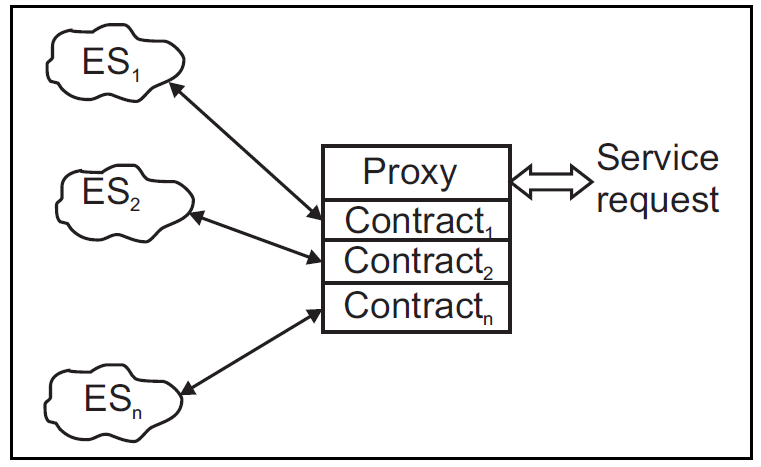
\includegraphics[width=0.3\textwidth]{../images/implementation/proxy_arch.png}
		} 
		\subfloat[Translator approach provides logical conversion]{
			\label{fig:tranlator_arch}
			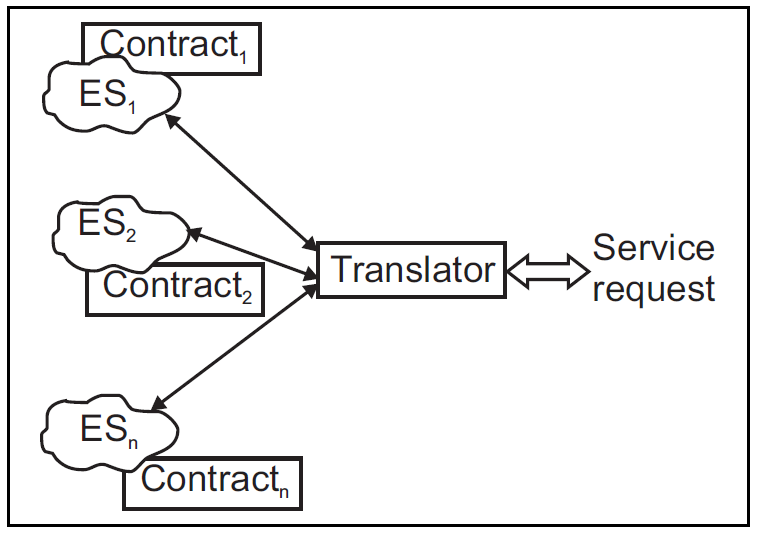
\includegraphics[width=0.3\textwidth]{../images/implementation/translator_arch.png}
		}
		\subfloat[Full approach where embedded systems directly provide services for the environment]{
			\label{fig:full_arch}
			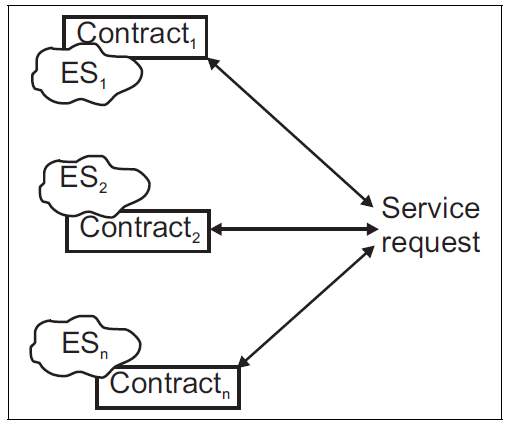
\includegraphics[width=0.3\textwidth]{../images/implementation/full_arch.png}
		} 
		       
        \caption{Possible connection architectures for the embedded services}
        \label{fig:connection_architectures}
\end{figure}




Proxy is a device which is between the client and the embedded service. It
provides services to the client and in the same time can communicate with
embedded system using closed protocols. Proxy device stores service contracts
onboard and know all specifications of connected embedded systems. 

Translator approach is similar to the Proxy, but it covers devices with proprietary
logical communication. The underlying physical transport is common to client and
service provider. The main purpose of Translator is to convert messages that
come from clients into into a logical format that the embedded system
can understand. Service contracts are stored inside services on the other
embedded systems, not on Translator. Translator may not be a separate device and
it can be only a software module.

In the Full architecture client and service provider can directly connect to
each other without need of any device in the middle. 

Our coffee machine system use closed proprietary protocol inside, but all
communication messages are transferred over standard serial line. This is more
similar to Translator approach, but there is one problem in implementing such
architecture. We cannot directly store service contract inside coffee machine
system. Coffee machine internal architecture and implementation does not allow
us to store any additional code for implementing service functionality. Internal
processor is utilized enough and there are no resources for anything else except
controlling coffee machine. In addition, the company did not
provided to me a specification of internal communication mechanism . There
are several microcontrollers inside that are controlling different machine
parts.
They provided  only the external interface communication protocol to me,
therefore my implementation is more similar to Proxy approach, where contracts are stored inside Proxy machine
and Proxy is a separate physical device.
\autoref{fig:general_system_arch} shows the general architecture of created
system.

\begin{center}
 \begin{figure}[h]
	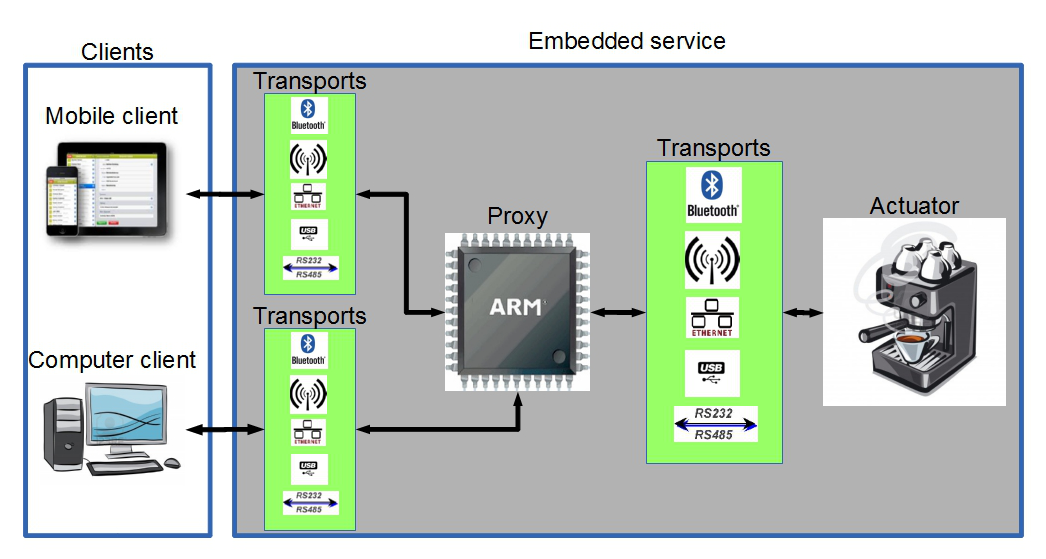
\includegraphics[width=\textwidth]{../images/implementation/system_arch.png}
	\caption{General system architecture }
	\label{fig:general_system_arch}
 \end{figure}
\end{center}

This is a traditional client-server approach where clients ( mobile or desktop)
send the requests to the server( Proxy embedded device) over some network and
physical transport( Bluetooth, various radio frequency connections, ethernet,
\gls{USB}, serial line, \ldots). Proxy server is connected to the controlled device 
(marked on the figure as Actuator), which is the coffee machine in this example
application.

There can be different clients and proxy can control and monitor various
devices, but connection scheme 
\(
{Client}\leftrightarrow{Transport}\leftrightarrow{Proxy}\leftrightarrow{Transport}\leftrightarrow{{Controlled~
or~monitored~device}} \)  is essential.

In this application mobile clients are connected through Bluetooth wireless. 
Each client may be connected using supported by the proxy device transport.
The proxy is connected to coffee machine by wires and serial line. 

Next section covers the internals of Proxy device.



\newpage
\subsection{Implementation of the embedded server}
Here will be STM32 server implementation.


\subsubsection{Authentication and Authorization}
\paragraph{Need of security}
Users are essential part of every system. System shold be designed with
a requirement, that there will be at least one user. System without any users
does not make sense. Usually information systems have lots of users with
different roles. There should be an system administrator - the most authorized individual
in the system, managers and normal users. System should distinct them all
somehow.

Another requirement is system and information security. System may contain
sensitive data, that should not be available to general users. In case of remote
services there are some services that are not open. These services or some
of their parts are require some identity to pass through. 

Let's take a usual website as example. Common website has at least three
different user roles:
user or guest, content publisher and system administrator. Last two roles may be
joined together, but in general content publishers do not do system maintenance, they
just work with content of webpages. There may be more different roles, but these
are the main ones. Imagine you open a web page and you see the content. You
follow the links and surf the web site. If you want to change something, for
example you do not like the design or some words on web page were misspelled,
you need to find special place where you can input your \textbf{credentials} and
get into the system. This will happen only if you have proper
\textbf{permission} to do that. When you get inside you are still not able to do
anything due to lack of privileges. For example you cannot turn of the
webserver or disable the your website. There may be lots of different roles and
responsibilities in the system and each role has limited access to system
resources.

Embedded device as a service may be similar to system example above. Device may
have some limited use cases, that are not available to not authorized service
clients. This may be internal information retrieving, some  device
manipulation functions (turn on/off something, delete/remove something from the
system, change of system preferences). Some device functionality may be
available only for limited people, for example system owner. The real life example of such system is the wireless
router. Router clients are other computers, they can send and receive network
packets. Router uses wireless security protocols, which permit unauthorized
access. Even if you are connected to a secure access point, you are not able to
change system settings. You should have admin permission (password) to manage
the system. This kind of system, like many embedded systems, is made for one
purpose. Router purpose is to provide access for the network. You also can
remember lots of similar systems, that use authorized access. Nowadays it is not new to get
remotely into some device and to change internals, but embedded system
integrations are still not so common. Imagine near future, you are sitting at
work and thinking to go home. After a long day you became really hungry. You
take your smartphone and connect to your remote wireless fridge service at home. You type
your password and get list of all food in your fridge. Now you know what you
need to buy and the real candidates to be throwed to the rubbish bin. You adjust
power in some fridge area and your beer will be very cold when you get home. Is
it just a dream? Is it really hard to realize using present time technologies?


The main problem here is the security. Nowadays lots of communication between
different systems goes through the wireless channel. Radio link is also
available to your neighbour behind the wall. Generally, you do not want to
broadcast what is in your fridge or to give ability to connect to your air
conditioning service. Therefore you need to use some authentication scheme for
your service.

\paragraph{Authentication protocols}

Authentication is any process by which you verify that someone is who they claim
they are. (https://httpd.apache.org/docs/2.2/howto/auth.html)

Humanity has already invented a lot of different authentication techniques. 

The ways in which someone may be authenticated fall into three
categories: (http://en.wikipedia.org/wiki/Authentication)
\begin{itemize}
  \item the ownership factors: Something the user has (e.g., wrist band, ID
  card, security token, software token, phone, or cell phone)
  \item the knowledge factors: Something the user knows (e.g., a password, pass
  phrase, or personal identification number (PIN), challenge response (the user must answer a question), pattern)
  \item the inherence factors: Something the user is or does (e.g., fingerprint,
  retinal pattern, DNA sequence (there are assorted definitions of what is sufficient), signature, face, voice, unique bio-electric signals, or other biometric identifier).
\end{itemize}

Authentication may be one way (only client is checked for validity) and two way
( both client and server check each other). Some systems  may requre to use
different security factors together: you say password, provide ID card and show
you fingerprint There are also available many standart authentication protocols.
If you start searching you will probably find similar list:
\begin{itemize}
  \item Transport Layer Security (TLS)
  \item Extensible Authentication Protocol (EAP)
  \item Password authentication protocol (PAP)
  \item Challenge-Handshake Authentication Protocol (CHAP)
  \item Password-authenticated key agreement
  \item Remote Authentication Dial In User Service (RADIUS)
  \item Kerberos
  \item Lightweight Extensible Authentication Protocol (LEAP)  
\end{itemize}

Choosing suitable protocol is not trivial problem. There is no any case general
protocol.  Most of them are designed to interconnect big computers inside a
network. Mostly they operate on transport and application level and use TCP/IP
protocol stack.

All these protocols could be devided into these groups:
\begin{itemize}
  \item Protocols that transmit the secret over the network. (For example
  Password authentication protocol). These protocols are not secure.
  \item Protocols that not send secrets and provide authentification through
  sending messages. (CHAP and Password-authenticated key agreement).
  \item Protocols that require a trusted third party.  
\end{itemize}

Protocols of first type have been deprecated because of security reasons. They
send sensitive data over the network and everyone else between two nodes can
catch this data.

Second group of protocols was invented because the first group was unable to
provide proper level of security. Link between client and server (two parties)
does not contain pure information about the secret. Parties use cryptography and
send encrypted messages to each other. Finally they authenticate each other when there is enough information gathered to validate the authority.

Last group uses trusted third party authority to check each other. There is
assumption that all three parties should have connection between each other. Embedded device during
client authentification needs to connect some server and ask for a secret. Third
party should always have a high authority, two other parties should trust him.
This scheme should be used in case of high security requirements.



Choosing of right authentication protocol in general should depend on application. Sometimes, there even will be enough to send plain text passwords over the network. Engineer should analyze all hazards during system design process.

Lifecycle of an embedded system is more longer than livecycle of average personal computer. Application specific controller  may run for decades and it will be still functional.
Choosed security algorithm may be not secure enough after some years. Some vulnerabilities can be discovered during that period. 
Computational power of modern processors raises every year and  secure encryption may be cracked during some seconds in the future.
There is no 100% secure system, everything is breakable. 

Your system security should have such encryption, that provides proper security level to your application data and can not be cracked quickly.

Another aspect is the complexity of cryptography algorithms. Embedded devices are usually small low power devices with limited computation abilities. Not every algorithm suits well. It should be quick and in same time be secure.

Code footprint here.

Challenge-Handshake Authentication Protocol will be used in this work




 One solution is to use closed encrypted proprietary
protocol and be calm, but as it was mentioned earlier, it limits the possibility of integration
between other embedded systems. It this case all of your devices should support
that protocol and you choise of different hardware is limited. Proprietary
protocols are often vendor-specific, code is closed, documentation is not free
and all it works only with the proprietary devices from the manufacturer.


\begin{center}
 \begin{figure}[h]
	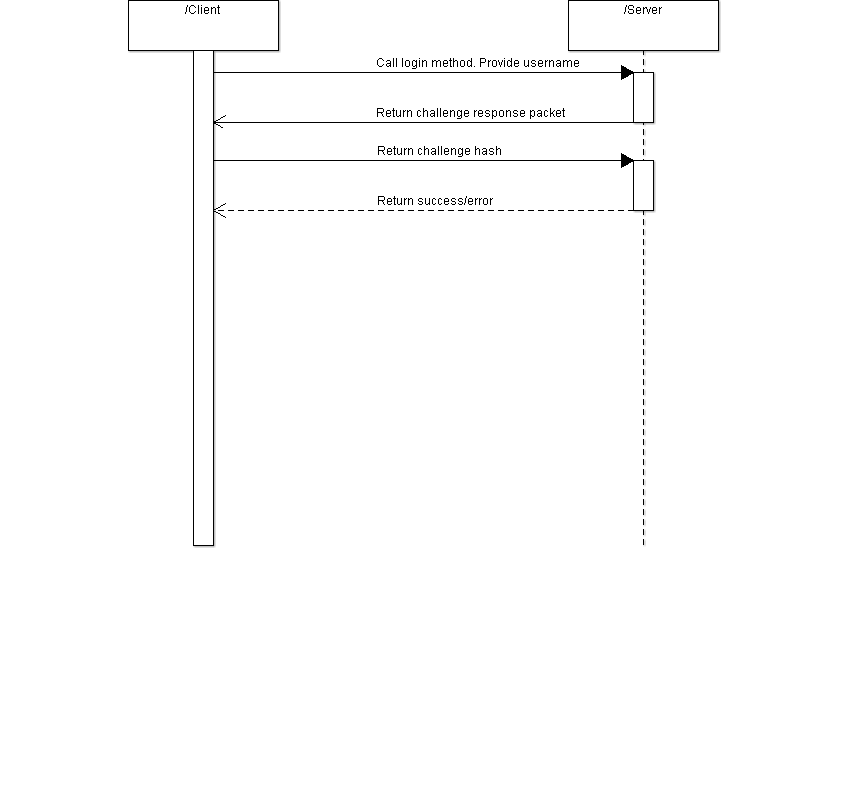
\includegraphics[width=\textwidth]{../images/implementation/embedded_server/SequenceDiagram.png}
	\caption{Client authentification process}
	\label{fig:embedded_server_login_auth}
 \end{figure}
\end{center}




\newpage
\subsection{General purpose client library implementation}
\label{sec:java_library}

\subsubsection{The technology used}
This section will define a client side of embedded service application.
JSON-RPC messages are used as the main application protocol.
Client part should also support all these features that server offers.

\autoref{fig:rpc_call} showed the main architecture of RPC.
RPC client   application usually consists of two modules: client application code
and client RPC stub, that communicates with remote server.
Client calls usual methods on a stub and the code in a stub handles all
the communication magic, it sends requests, receives responses, serialize and
diserialize data objects.

There were already some examples of a small RPC application (see listings
\ref{lst:rpc_server_python_example} and
\ref{lst:rpc_client_python_example})
Our system requirements and environment does not allow to use Python programming
language.
The client application in this work is written for Google Android smartphone
platform, which has a \gls{JVM} virtual machine inside, and the Java programming
language is used.

Java is very popular programming language which is based on \textit{"Write
once, run anywhere"} philosophy. This means a programmer can develop code on a
PC and can expect it to run on any Java enabled hardware, from small embedded systems
to huge server mainframes. 
This is quite mature programming language with lots of libraries and already
written code that solves different problems. For example, see a list Java tools
for JSON at \url{http://www.json.org/}.

The Android system uses Java as one of the main programming language. 
Most programs for android are written using Java and Google provides good
Android development tools for Java programming language.
The Android client application will be covered in the next section, while this one will describe the client
stub library which is written in Java. 
This code can be executed on every hardware that is supported by Java virtual
machines. Application architecture in this projects is based on the ideas of
extensibility and portability and therefore Java is a good choice to start.

I have implemented an universal library for the RPC communication with the
previously described embedded service. That library is easy to add to any Java
project and start to develop a new control application. 
It can be extended to add some required functionality.
 
\subsubsection{Library structure}

The library interface should be identical to a service interface description
or service contract. The JSON service descriptor from the
\autoref{sec:appendix_service_contracts} has enough information to create a
binding library to that embedded service.

This client code can be realized in two different ways: static and dynamic binding.
The library described here, is a static binding library, because it has an already 
defined interface class and client methods are known at the compile time.

Dynamic libraries can determine available server methods at the runtime. Client
library may connect to a server and receives a list of operations. For example JSON
service contract that is used in this work, can be obtained and parsed at the runtime. Dynamic proxy
class can be created from received list of methods and methods can be called
only by a name without the compile time checking. Client may know only a method
name or a part of that name and decide while application is running, which
methods to call. Domain keywords for Java are: \textit{reflection}, \textit{dynamic proxy
class}, \textit{duck typing}. 
The Python example above uses this approach and
you can retrieve list of available methods from server by calling
\texttt{listMethods()} on a \texttt{ServerProxy} object. 
This technique is more suitable for dynamically typed programming languages. 

I preferred to make more robust and simple solution. I created a Java
interface class with all methods that server has. 
The definition of the main interface classes in the library is provided below.

\begin{listing}[H]
\begin{minted}[frame=lines,
               framesep=2mm]{java}
public interface Service {

    // connect methods
    void connect(Reader inputReader, Writer outputWriter);
    boolean isConnected();
    void disconnect();

    public void start();
    public void stop();
    public boolean isRunning();

    boolean addListener(RPCServiceListener listener);
    boolean removeListener(RPCServiceListener listener);

    void setTimeoutMs(long timeoutMs);
    long getTimeoutMs();

    void setRequestProcessor(RequestProcessor requestProcessor);
    RequestProcessor getRequestProcessorByType(
	    Class requestProcessorClass,
	    Object... params);
}               
               
public interface CoffeeMachineService extends Service {
    ServiceContract getServiceContract();
    
    Map<String, Object> getInfo();
    
    // products
    List<Product> getProducts();
    Product.Status orderProduct(int productId);
    Product.Status cancelProduct(int productId);
    Product.Status getProductStatus(int productId);
}
\end{minted}
\caption{RPC client main interface class}
\label{lst:rpc_client_interface_class}
\end{listing}

Some object oriented design techniques are used here to get a more abstract code. 
\texttt{CoffeeMachineService}  extends another
interface \texttt{Service}, which has method that are common to every RPC
service.
\texttt{CoffeeMachineService} interface contains only coffee machine related methods and
inherits other methods from the parent class.

Client can use these classes in the application code and does not need to know
the implementation details. To start using it client needs to create an instance
of \texttt{JsonRpcCoffeeMachineService} ( the implementation of
\texttt{CoffeeMachineService} interface), connect it to \texttt{Reader} and \texttt{Writer} stream objects and after that  user can call RPC methods.

\paragraph{Character encoding} ~\\
Java programming language has the abstraction of \texttt{Reader} and
\texttt{Writer}. These are character stream interfaces that allow to write or
read characters to/from underlying information sources. JSON-RPC is a text
based protocol and we only need to handle character data in our application, but
not binary data.\texttt{Reader} and \texttt{Writer} are parents of
\texttt{InputStreamReader} and \texttt{OutputStreamWriter}, which are bridge
from byte streams to character streams. They transfer bytes to characters and
back using a specified character set\footnote{the mapping between characters and sequences of bytes}.
JVM internally stores characters as 16-bit Unicode variables, but in other
systems character can be:  an US-ASCII seven-bit value, UTF-8 multi-byte
encoding, Extended Binary Coded Decimal Interchange Code (EBCDIC) 8-bit
character encoding and others. Character encoding needs to be specified for
\texttt{InputStreamReader} and \texttt{OutputStreamWriter} in order to convert
data properly. We cannot use byte streams in our library because we cannot
predict in which encoding character data will be received from the data byte
source. It might happen that some byte will have different meaning from what we
expect. Therefore we use an abstraction of \texttt{Reader} and
\texttt{Writer} here.

Client of our library should receive an \texttt{InputStream}  object (operates
with byte streams) from somewhere, provide valid character encoding and create
an \texttt{InputStreamReader} from \texttt{InputStream}, and pass it to
\texttt{connect()} method of the RPC library. The source of an
\texttt{InputStream} may be the array of bytes in the memory, a file on the
disk, a network socket or even String objects. In general words, client should
decide where from data bytes should come, where they need to be written, and
wrap these bytes into character streams.

\paragraph{Message encoding} ~\\

This library assumes that received characters are encoded using
netstrings\footnote{ \texttt{<LENGTH>:<DATA>,} format, for more details see
\autoref{sec:netstrings} } message encoding.
\texttt{MessageReader} class in the library has the implementation of similar finite
state machine parsing algorithm, that was used in the embedded server implementation.
It reads the netstrings encoded messages, extracts the data from them and sends extracted characters to
\texttt{MessageHandler} for processing.


The \texttt{MessageWriter} class composes a valid netstring message and  uses the provided
by a client \texttt{Writer} object to write that message to the destination.
\texttt{MessageWriter} receives JSON  objects,converts them into a String data, wraps them
in a netstring message and sends this character data to the destination.

\paragraph{JSON serialization and the JSON-RPC} ~\\

This JSON-RPC client is based on the \texttt{jsonrpc2-base} library from
Vladimir Dzhuvinov (\url{http://software.dzhuvinov.com}).
This library provides a ready classes for handling JSON-RPC requests and
responses.
\autoref{tbl:jsonrpc2-base_methods} shows the entire lifecycle of a RPC call.



\begin{longtabu} to \linewidth {|p{1cm}|p{1.5cm}|X|p{8cm}|}
 	\caption{jsonrpc2-base library RPC methods \cite{jsonrpc2-base}}
	\label{tbl:jsonrpc2-base_methods} 	 	
\hline 
\multicolumn{1}{|l|}{\textbf{Step}} & 
\multicolumn{1}{l|}{\textbf{Side}} &
\multicolumn{1}{l|}{\textbf{Action}} &  
\multicolumn{1}{l|}{\textbf{Used methods}} \\ 
\hline 
\endfirsthead

\multicolumn{4}{l}%
{{\bfseries \tablename\ \thetable{} -- continued from previous page}} \\
\hline 
\multicolumn{1}{|l|}{\textbf{Step}} & 
\multicolumn{1}{l|}{\textbf{Side}} &
\multicolumn{1}{l|}{\textbf{Action}} &  
\multicolumn{1}{l|}{\textbf{Used methods}} \\ 
\hline 
\endhead

\hline \multicolumn{4}{|r|}{{Continued on next page}} \\ \hline
\endfoot

% \hline \hline
\endlastfoot

		1 &
		Client &
		Create a new request &
		\texttt{JSONRPC2Request()}	
		
		\tabularnewline
		\hline
		2 &
		Client &
		Serialize request to string and send &
		\texttt{JSONRPC2Request.toString()}	
		
		\tabularnewline
		\hline
		3 &
		Server &
		Parse received string back to request object &
		\texttt{JSONRPC2Request.parse()}
		
		\tabularnewline
		\hline
		4 &
		Server &
		Get the request data &
		\texttt{JSONRPC2Request.getMethod()}\newline
		\texttt{JSONRPC2Request.getParamsType()}\newline
		\texttt{JSONRPC2Request.getPositionalParams()}\newline
		\texttt{JSONRPC2Request.getNamedParams()}\newline
		\texttt{JSONRPC2Request.getID()}\newline
		
		\tabularnewline
		\hline
		5 &
		Server &
		Create a response &
		\texttt{JSONRPC2Response()}
		
		\tabularnewline
		\hline
		6 &
		Server &
		Serialise response to string and send back &
		\texttt{JSONRPC2Response.toString()}
		
		\tabularnewline
		\hline
		7 &
		Client &
		Parse received string back to response object &
		\texttt{JSONRPC2Response.parse()}
			
		\tabularnewline
		\hline
		8 &
		Client &
		Check the response for success, get the result/error &
		\texttt{JSONRPC2Response.indicatesSuccess()}\newline
		\texttt{JSONRPC2Response.getResult()}\newline
		\texttt{JSONRPC2Response.getError()}\newline

		
		\tabularnewline
		\hline
	%\end{tabularx} 

\end{longtabu}

\texttt{jsonrpc2-base} is able to serialize Java data types to JSON objects
Listing \ref{lst:jsonrpc2-base_serialization} shows how RPC request object is
created from the standard Java data types and \autoref{tbl:json_java_mapping}
shows how JSON to JAVA mappings are done.

\begin{listing}[H]
\begin{minted}[frame=lines,
               framesep=2mm]{java}
// The remote method to call
String method = "makePayment";

// The required named parameters to pass
Map<String,Object> params = new HashMap<String,Object>();
params.put("recipient", "Penny Adams");
params.put("amount", 175.05);

// The mandatory request ID
String id = "req-001";

// Create a new JSON-RPC 2.0 request
JSONRPC2Request reqOut = new JSONRPC2Request(method, params, id);

// Serialize the request to a JSON-encoded string
String jsonString = reqOut.toString();

// jsonString can now be dispatched to the server...
\end{minted}
\caption{RPC request creating from Java standard data types \cite{jsonrpc2-base}}
\label{lst:jsonrpc2-base_serialization}
\end{listing}


\begin{table}[h]
	\centering	
	\caption{{JSON} \ding{214} {Java} data type mapping in
	\texttt{jsonrpc2-base} library \cite{jsonrpc2-base}}
	\label{tbl:json_java_mapping}
	\begin{tabularx}{0.5\textwidth}{|X|X|}
		\hline
		\textbf{JSON} & \textbf{Java} 	 	\\ \hline	    
		true or false & java.lang.Boolean 	\\ \hline	    
		number & java.lang.Number		 	\\ \hline
	   	string & java.lang.String		 	\\ \hline		
		array & java.util.List		 	\\ \hline
		object & java.util.Map			 	\\ \hline
		null & null		 	\\ \hline			  
	\end{tabularx} 

\end{table}

\paragraph{Data flow} ~\\

This paragraph describes the client stub library RPC call in details. 
Although \texttt{jsonrpc2-base} has classes for handling JSON-RPC message
objects, it does not provide any client functionality. 
We need to write a request handling logic to support the communication with
hardware embedded service.

When client of our library calls any method on \texttt{CoffeeMachineService}
class this method starts to prepare a new request. Service interface
implementation add necessary parameters to RPC request (name, method
parameters, an id), and sends it to request processor.

The whole RPC call process visualized at the \autoref{fig:rpc_call_java} 


\begin{sidewaysfigure}
\centering
\scalebox{0.4}
{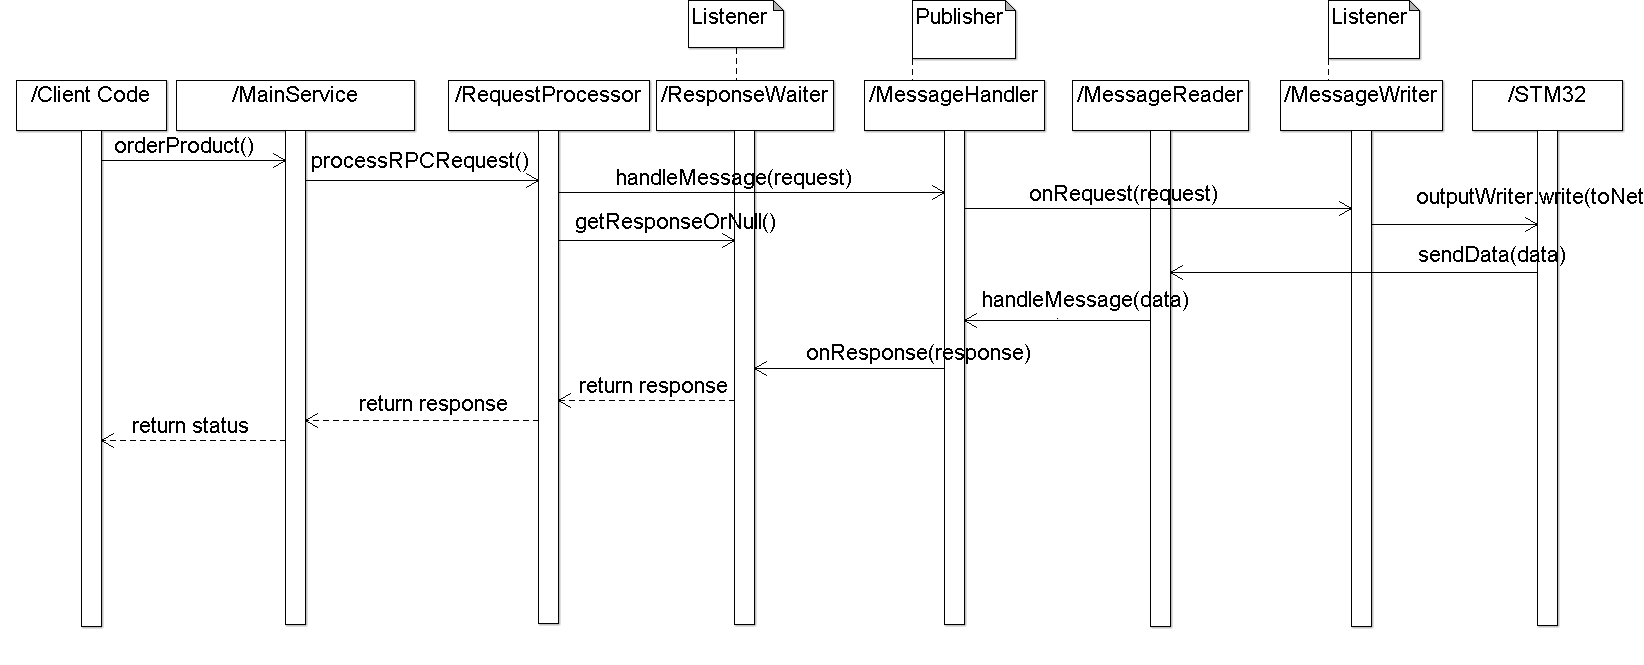
\includegraphics{../images/implementation/java_flow_diagram.png}}
\caption{RPC call in the client stub library}
\label{fig:rpc_call_java}
\end{sidewaysfigure}

\texttt{RequestProcessor} is a simple object with a ~\texttt{Object
processRequest(Object request)} method which encapsulated request processing
logic. Strategy design pattern is implemented here. 
Each request can be processed in a many various ways.
Some methods  have slow execution  on the server and require bigger timeout time
on the client side. Another methods could fail and additional error handling
logic is required. This design methods help to define different  
request handling strategies and apply them at the runtime.
For example the \texttt{getProducts()}  method has very short response time,
because it does not trigger any events on the coffee machine.
Proxy device just returns a list of products from memory storage. 
Another method, the \texttt{orderProduct()}, needs additional communication and
verification of parameters. 
These two methods may have two different algorithms of processing client RPC
request, while programming interface needs to stay fixed.

There is only one strategy for the \texttt{RequestProcessor} implemented yet.
This processor sends a request to a message handler only ones and starts to wait
for a response from a \texttt{RequestWaiter} help class.
After some timeout it returns the result or a \texttt{null} value if there was
not  any response received.

Message writer module of the client stub implements the
\texttt{RPCServiceListener} (pay attention to the 
\texttt{addListener()} and \texttt{removeListener()} methods in listing
\ref{lst:rpc_client_interface_class}) interface. 
This is a \textbf{publish-subscribe mechanism} used in this library for  event
handling.
Service implementation contains a list of service listeners, who are listening
for various RPC messages. 
Listing \ref{lst:event_listener_publisher_interfaces} contains a list o messages that can
be captured by the \texttt{RPCServiceListener}. It also contains a interface of a
class that publishes internal system events.

\begin{listing}[H]
\begin{minted}[frame=lines,
               framesep=2mm]{java}
public interface RPCServiceListener {
    void onRequest(RPCRequest request);
    void onResponse(RPCResponse response);
    void onNotification(RPCNotification notification);
    void onUnknownMessage(String messageText);
}

public interface MessageHandler {
    void handleMessage(String msg);
    void handleMessage(RPCRequest request);
    void handleMessage(RPCNotification notification);
    void handleMessage(RPCResponse response);
}
\end{minted}
\caption{RPC event listener and event publisher interfaces}
\label{lst:event_listener_publisher_interfaces}
\end{listing}

Message writer thread listens for the \texttt{onRequest()} and
\texttt{onNotification()} events. It starts to write request message data to
remote embedded device using the output character \texttt{Writer}  when these
methods are triggered by the request publishers.

System event methods are triggered by a
\texttt{MessageHandler}. This is a small routing class that decides where to put
moving requests, notification, responses and errors according to their types. 
For example, if \texttt{handleMessage(RPCRequest request)} message handler
method is called from somewhere in the code, message handler publishes received
\texttt{RPCRequest} object to all subscribed listeners. 
Message handler calls \texttt{onRequest(RPCRequest request)} method on each
service subscriber and passes new \texttt{RPCRequest} as parameter.

Messages from the the remote device are read by a \texttt{MessageReader} class.
This class reads incoming netstring packets  and passes extracted data
to the \texttt{MessageHandler}. \texttt{MessageHandler} parses incoming JSON 
data and detects that this data type is a JSON-RPC response object. This
Response message becomes published for all listeners including the 
\texttt{ResponeWaiter} help class, who receives message and return it to
\texttt{RequestProcessor}. 


Now the \texttt{RequestProcessor} have received a response it was waiting for
and it can be returned to \texttt{MainService} class. Not the data from the 
response message can be extracted  and remote call result may be returned
to a client code, from where it was initially called.


This is how JSON-RPC messages flow inside service client library.

It might seem quite complicated, but it has lots of advantages. 
Using a publish-subscribe mechanism you might add  multiple event listeners to
the system very easily. 
For example if you need a request logger, you create a class which implements a
\texttt{RPCServiceListener} interface and register it in a main service class 
by calling special methods. Now your logger can listen all RPC
messages and log the information about them.

\paragraph{Conclusion} ~\\

This library can be used in the client application code as the abstract interface of a remote coffee machine.
It makes programming of client code more elegant and easy.
System programmer does not need to develop RPC related code, he can simply use this interface in his projects.
The only necessary step is the connection of a service instance class to the data input and output character streams.
This library uses the netstrings  character data encoding, which is a very simple way how to transfer character data messages.
The whole design is based on the JSON-RPC communication protocol.




%\newpage
\subsection{Implementation of Android client example applications}

The prototype of client-server application was designed during this research project.
The application program was executed on the Google Android operating system powered hardware.


Main idea of this application is the remote wireless control of some electronic device. 
The controlled device example here is a coffee machine, that has some functions like preparing a cup of coffee.
We needed that these functions became available for remote control.

The developed application is a small application with trivial user interface, which allows to prepare products by selecting a product from a small catalogue. 
The screen shot of a ready application is provided  in the \autoref{fig:android_app_screen}

\begin{center}
 \begin{figure}[h]
	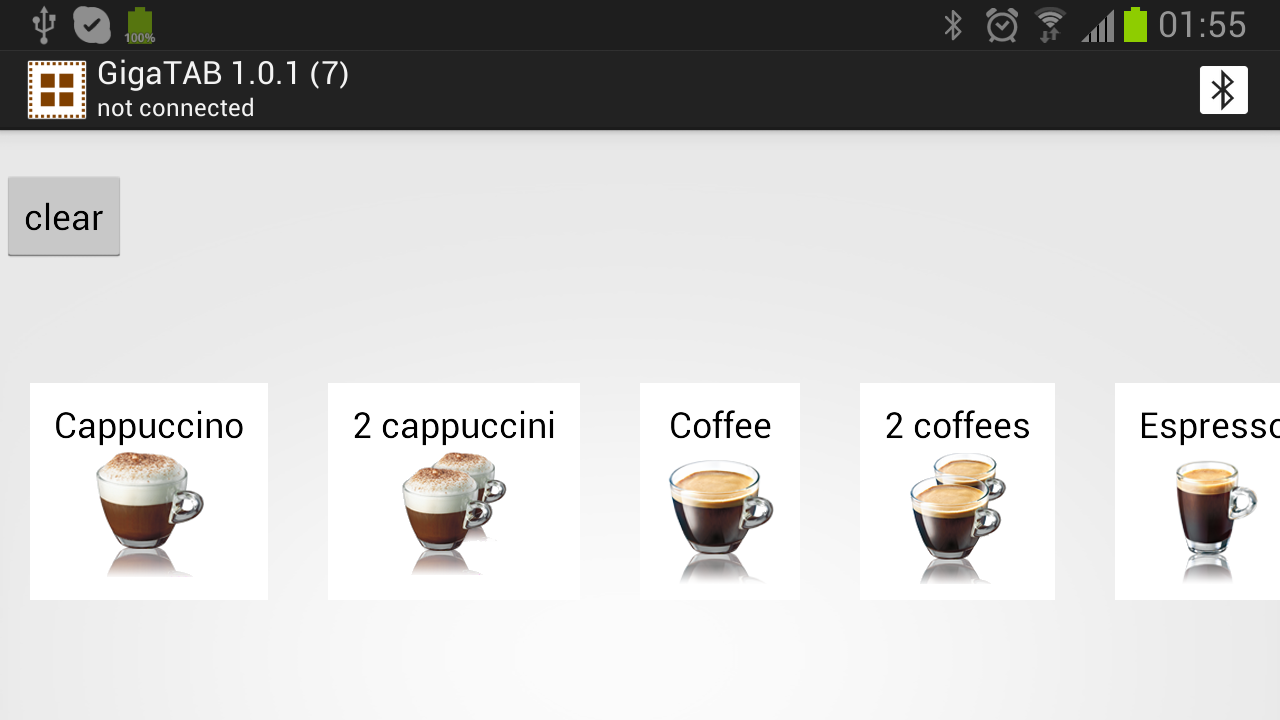
\includegraphics[width=\textwidth]{../images/implementation/android_app_screen.png}
	\caption{Android application visual interface }
	\label{fig:android_app_screen}
 \end{figure}
\end{center}

The usage scenario starts from the connection to coffee machine.
There is a small button with Bluetooth icon in the top right corner of the application.
This button activates a device select dialog, where you can find a remote device by name and MAC address and connect by selecting it in the list.
When connection is established some available products become showed in the horizontal list layout.
It is able to point to each of these products and open a dialog box with detailed information about each product.
User can start coffee preparing from that dialog.
While operation is in progress, it is still possible to cancel the product preparing operation.

I will not cover in details the whole process of the user interface and application creation.
This is out of the scope of this research work and it requires some additional domain knowledge. 
You need to get familiar with Google Android development tools,
read a documentation course, follow the tutorials and study by doing.
There are available lots of application examples and it is not very hard to produce a similar application.
This application is partially based on the Bluetooth chat communication example from the Android Software development kit.

Whole communication is performed over wireless Bluetooth protocol.
It is assumed, that Bluetooth is the abstract transport that can send data bytes over radio link.
The Android Bluetooth API functions can search to nearby Bluetooth devices and provide you a list of \texttt{BluetoothDevice} objects.
You can find your wireless device in that list and tell the Android OS to connect to that device. 
This device list is also used to fill a device choosing graphical dialog described before.

When devices get connected  it is able to receive a communication socket object and get a standard \texttt{java.io.InputStream} and \texttt{java.io.OutputStream} from that.
This is a final step of establishing the communication and it is able to transfer data over received stream objects.


The client RPC library is connected to these streams and it is able to communicate with a remote device over the wireless serial interface.
RPC calls may be started right after application gets connected to the Bluetooth input and output streams.


Now it is up to your imagination how to use and extend this remote embedded service.
You can implement any rich functionality and create whatever complex system you want or your hardware resources allow you.
This extensible service oriented embedded architecture allows you to do so.
